\documentclass[handout]{beamer}
 
\usepackage[utf8]{inputenc}
\usepackage{mathtools}
\usepackage{tikz}
\usetikzlibrary{calc}

\usetheme{CambridgeUS}
% \useoutertheme{split}
\setbeamertemplate{title page}[default][colsep=-4bp,rounded=true]

% only inlcude the current secition in the header
\AtBeginSection{
    \begin{frame}
        \tableofcontents[sections=\value{section}, sectionstyle=show/show]
    \end{frame}
}

%Information to be included in the title page:
\title{Public Key Primitives}
\author{Rohit Musti}
\institute{CUNY - Hunter College}
\date{\today}
 
\begin{document}
 
\frame{\titlepage}

% Outline frame
\begin{frame}{Table of Contents}
  \tableofcontents
\end{frame}


\section{Overview}

% Motiviating Key Exchange Problem
\begin{frame}{Public Key Exchange Motivation}
    \begin{itemize}
        \item \pause Consider our protagonists: Alice and Bob. They have never met in person and are speaking over the phone to coordinate a blind date!
        \item \pause They want to make sure their date location is secret from any eavesdroppers listening to their phone line.
        \item \pause They took introduction to cryptography and decide that they want to generate a shared secret \(c\) unknown to any adversary.
        \item \pause This requires that if the eavesdropper takes the transcript of their phone call, they are not able to generate the secret \(k\) 
    \end{itemize}
    \pause NOTE: no requirements for integrity (no protection from man in the middle) and the protocol is fully anonymous (no way to verify that Alice and Bob are talking to one another)
\end{frame}

% Key Exchange Attqck
\begin{frame}{Anonymous Key Exchange Attack Game}
    \begin{tikzpicture}
      \pause
        \node[draw] (AdversaryA) at (-3, 2) {\(\mathcal{A}\)}; 
        \draw[thick] (AdversaryA) -- ++(0, -4); 
        \draw[thick] (AdversaryA) -- ++(-2, 0);
        \draw[thick] (-3, -2) -- ++(-2, 0);
      \pause
        \node[draw] (ChallengerA) at (4,2) {\(\mathcal{C}\)}; 
        \draw[thick] (ChallengerA) -- ++(0, -4);
        \draw[thick] (ChallengerA) -- ++(2, 0);
        \draw[thick] (4, -2) -- ++(2, 0);

      \pause
        \node[draw=none,fill=none,anchor=west, font=\footnotesize] (choice0) at ($(ChallengerA) + (.25,-1)$) {run protocol};
        \node[draw=none,fill=none,anchor=west, font=\footnotesize] (choice0) at ($(ChallengerA) + (.25,-1.3)$) {generate \(k\)};

      \pause
        \draw[->,thick] ($(ChallengerA)+(-0.25,-2)$) -- ($(AdversaryA)+(0.25,-2)$) node [pos=0.5,above,font=\footnotesize] {protocol transcript: \(T_p\)};

      \pause
        \draw[->,thick] ($(AdversaryA)+(-1,-4.15)$) -- ($(AdversaryA)+(-1, -5)$) node [pos=0.5,right,font=\footnotesize] {k'};

      \pause
        \node[draw=none,fill=none,anchor=east, font=\footnotesize] (choice0) at ($(ChallengerA) + (0, -6)$) {if \(k' = k\), then the adversary wins};
      \end{tikzpicture}
\end{frame}

\begin{frame}{Weaknesses in this Security Notion?}
    \begin{enumerate}
        \item \pause Assumes adversary will not tamper with protocol \pause
        \item Assumes that adversary cannot simply guess parts of \(k\) (i.e. no uniform randomness distinguishability requirement) \pause
        \item No identity verification
    \end{enumerate}
\end{frame}

\section{Trapdoor Functions}

% Trapdoor Functions
\begin{frame}{Trapdoor Functions}
    \begin{itemize}
        \item \pause Trapdoor functions are one way functions that have a "trapdoor" that allows someone armed with a secret to reverse the otherwise unreversible function
        \item \pause Three functions over \((\mathcal{X}, \mathcal{Y})\): a generator, a function, and an inverter 
        \begin{itemize}
            \item \pause \(G\): probabilistic generator  (\(pk, sk) \xleftarrow[]{R} G()\)
            \item \pause \(F\): determinstic function \(y \xleftarrow[]{} F(pk, x)\) 
            \item \pause \(I\): determinstic function \(x \xleftarrow[]{} I(sk, y)\) (should be hard w/o \(sk\))
        \end{itemize}
        \item \pause correctness: \(\forall (pk, sk): I(sk, F(pk, x)) = x\)
    \end{itemize}
\end{frame}

% Trapdoor Key Exchange 
\begin{frame}{Trapdoor Key Exchange}
    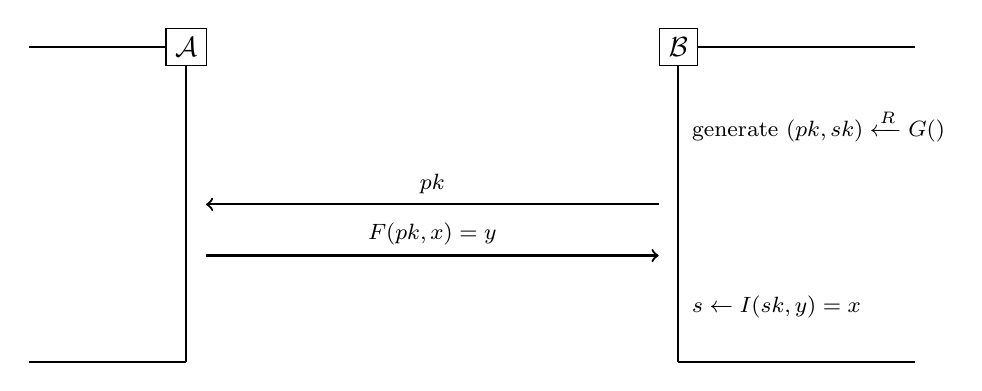
\begin{tikzpicture}
      \pause
        \node[draw] (AdversaryA) at (-3, 2) {\(\mathcal{A}\)}; 
        \draw[thick] (AdversaryA) -- ++(0, -4); 
        \draw[thick] (AdversaryA) -- ++(-2, 0);
        \draw[thick] (-3, -2) -- ++(-2, 0);
      \pause
        \node[draw] (ChallengerA) at (3.25,2) {\(\mathcal{B}\)}; 
        \draw[thick] (ChallengerA) -- ++(0, -4);
        \draw[thick] (ChallengerA) -- ++(3, 0);
        \draw[thick] (3.25, -2) -- ++(3, 0);

      \pause
        \node[draw=none,fill=none,anchor=west, font=\footnotesize] (choice0) at ($(ChallengerA) + (.05,-1)$) {generate \((pk, sk) \xleftarrow[]{R} G()\)};

      \pause
        \draw[->,thick] ($(ChallengerA)+(-0.25,-2)$) -- ($(AdversaryA)+(0.25,-2)$) node [pos=0.5,above,font=\footnotesize] {\(pk\)};

      \pause
        \draw[->,thick] ($(AdversaryA)+(0.25,-2.65)$) -- ($(ChallengerA)+(-0.25,-2.65)$) node [pos=0.5,above,font=\footnotesize] {\(F(pk, x) = y\)};

      \pause
        \node[draw=none,fill=none,anchor=west, font=\footnotesize] (choice0) at ($(ChallengerA) + (.05,-3.3)$) {\(s \leftarrow I(sk, y) = x\)};

      \end{tikzpicture}
\end{frame}

% Trapdoor Attack Game

\begin{frame}{Trapdoor Key Exchange Attack Game}
    \begin{tikzpicture}
      \pause
        \node[draw] (AdversaryA) at (-3, 2) {\(\mathcal{A}\)}; 
        \draw[thick] (AdversaryA) -- ++(0, -4); 
        \draw[thick] (AdversaryA) -- ++(-2, 0);
        \draw[thick] (-3, -2) -- ++(-2, 0);
      \pause
        \node[draw] (ChallengerA) at (3,2) {\(\mathcal{C}\)}; 
        \draw[thick] (ChallengerA) -- ++(0, -4);
        \draw[thick] (ChallengerA) -- ++(3, 0);
        \draw[thick] (3, -2) -- ++(3, 0);

      \pause
        \node[draw=none,fill=none,anchor=west, font=\footnotesize] (choice0) at ($(ChallengerA) + (.05,-1)$) {generate \((pk, sk) \xleftarrow[]{R} G()\)};
        \node[draw=none,fill=none,anchor=west, font=\footnotesize] (choice0) at ($(ChallengerA) + (.05,-1.45)$) {generate \(y = F(pk, x)\)};

      \pause
        \draw[->,thick] ($(ChallengerA)+(-0.25,-2)$) -- ($(AdversaryA)+(0.25,-2)$) node [pos=0.5,above,font=\footnotesize] {protocol transcript: \((pk, y)\)};

      \pause
        \draw[->,thick] ($(AdversaryA)+(-1,-4.15)$) -- ($(AdversaryA)+(-1, -5)$) node [pos=0.5,right,font=\footnotesize] {\(x'\)};

      \pause
        \node[draw=none,fill=none,anchor=east, font=\footnotesize] (choice0) at ($(ChallengerA) + (0, -6)$) {if \(x' = x\), then the adversary wins};
      \end{tikzpicture}
\end{frame}

\section{RSA}

% RSA Background
\begin{frame}{RSA Background}
    \begin{itemize}
        \item \pause Named after Ron Rivest, Adi Shamir, and Leonard Adleman at the Massachusetts Institute of Technology
        \item \pause Legend has it they got drunk on wine during passover at a student's house and came up with the system staying up all night
        \item \pause allegedly, the british intelligence agencies came up with a similar system a few years earlier but didn't think it was feasible with the current computers
    \end{itemize}
\end{frame}

% RSA Key Generation
\begin{frame}{RSA Key Generation}
    \begin{itemize}
        \item Key Generation
        \begin{enumerate}
            \item \pause pick an integer \(\ell > 2\) and an odd integer \(e > 2\) 
            \item \pause generate a random \(\ell\)-bit prime \(p\) s.t. \(gcd(e, p-1) = 1\)
            \item \pause generate a random \(\ell\)-bit prime \(q\) s.t. \(gcd(e, q-1) = 1\) and \(p \neq q\)
            \item \pause \(n \leftarrow pq\)
            \item \pause \(d \leftarrow e^{-1}mod (p-1)(q-1) \)
            \item \pause \(pk = (n, e)\) and \(sk = (n, d)\)
        \end{enumerate}
        \item \pause \(x \in \mathbb{Z}_n\)
        \item \pause \(F(pk, x) \coloneqq x^e \in \mathbb{Z}_n\) 
        \item \pause \(I(sk, y) \coloneqq y^d \in \mathbb{Z}_n\) 
    \end{itemize}
\end{frame}

% RSA Security
\begin{frame}{RSA Security}
    \begin{itemize}
        \item \pause given \(n\) the RSA Modulus, \(e\) the encryption exponent, \(d\) the decryption exponent, and \(y = x^e\), it is mathematically hard to calculate \(x\)
    \end{itemize}
\end{frame}

\section{Diffie-Hellman Key Exchange}

% Diffie Hellman History
\begin{frame}{Diffie-Hellman History}
    \begin{itemize}
        \item \pause Earned the authors a Turing award
        \item \pause Two Stanford Cryptographers Whitfield Diffie and Martin Hellman
        \item \pause Before this time, little cryptography work was done outside of the NSA and other intelligence agencies
        \item \pause NSA tried to limit their research after they published this public paper
        \item \pause NSA even sent letters to journal editors warning that authors of cryptography papers could be sentenced to prison time for violating laws around military weapon export
    \end{itemize}
\end{frame}

% Diffie Hellman History
\begin{frame}{Diffie-Hellman Key Exchange}
    \begin{itemize}
        \item start by sample two large primes: \(p, q\) s.t. \(q\) divides \(p - 1\)
        \item all math is done mod \(p\) (working in \(\mathbb{Z_p}\))
        \item since \(q\) divides \(p\), there exists a \(g\) s.t. \(g^q = 1\), this will serve as the generator for a Group (\(\mathbb{G}  \coloneqq {g^a: a = 0, ..., q - 1}\))
    \end{itemize}
\end{frame}

\begin{frame}{Diffie-Hellman Key Exchange}
    \begin{tikzpicture}
      \pause
        \node[draw] (AdversaryA) at (-3, 2) {\(\mathcal{A}\)}; 
        \draw[thick] (AdversaryA) -- ++(0, -4); 
        \draw[thick] (AdversaryA) -- ++(-2, 0);
        \draw[thick] (-3, -2) -- ++(-2, 0);
      \pause
        \node[draw] (ChallengerA) at (3.25,2) {\(\mathcal{B}\)}; 
        \draw[thick] (ChallengerA) -- ++(0, -4);
        \draw[thick] (ChallengerA) -- ++(3, 0);
        \draw[thick] (3.25, -2) -- ++(3, 0);

      \pause
        \node[draw=none,fill=none,anchor=east, font=\footnotesize] (choice0) at ($(AdversaryA) + (.05,-1)$) { \(\alpha \xleftarrow[]{R} \mathbb{Z}_q, u \leftarrow g^{\alpha}\)  };

      \pause
        \draw[->,thick] ($(AdversaryA)+(0.25,-1.65)$) -- ($(ChallengerA)+(-0.25,-1.65)$) node [pos=0.5,above,font=\footnotesize] {\(u\)};

      \pause
        \node[draw=none,fill=none,anchor=west, font=\footnotesize] (choice0) at ($(ChallengerA) + (.05,-2)$) { \(\beta \xleftarrow[]{R} \mathbb{Z}_q, v \leftarrow g^{\beta}\)  };

      \pause
        \draw[->,thick] ($(ChallengerA)+(-0.25,-2.65)$) -- ($(AdversaryA)+(0.25,-2.65)$) node [pos=0.5,above,font=\footnotesize] {\(v\)};

      \pause
        \node[draw=none,fill=none,anchor=west, font=\footnotesize] (choice0) at ($(ChallengerA) + (.05,-3.3)$) {\(w \leftarrow u^{\beta}\)};
        \node[draw=none,fill=none,anchor=east, font=\footnotesize] (choice0) at ($(AdversaryA) + (.05,-3.3)$) {\(w \leftarrow v^{\alpha}\)};

      \pause
        \node[draw=none,fill=none,anchor=east, font=\footnotesize] (choice0) at ($(ChallengerA) + (-1.5, -5)$) {\(w = v^{\alpha} = u^{\beta} = g ^ {\alpha \beta}\)};
      \end{tikzpicture}
\end{frame}

\begin{frame}{Diffie-Hellman Security}
    \begin{itemize}
        \item \pause Security rests on the difficulty of the discrete log problem
        \item \pause over a cyclic group \(\mathbb{G}\) it is mathematically hard to compute \(\alpha\) given \(g^\alpha\), where \(g\) is a generator of \(\mathcal{G}\)
        \item \pause this is further extended to: given (\(g^\alpha, g^\beta\)) where \(g\) is a generator, \(\alpha, \beta \xleftarrow[]{R} \mathbb{Z}_q\), it is hard to compute \(g^{\alpha\beta}\)
    \end{itemize}
\end{frame}

\end{document}